\documentclass[journal,twoside,web]{ieeecolor}
\usepackage{tmi}
\usepackage{cite}
\usepackage{amsmath,amssymb,amsfonts}
\usepackage{algorithmic}
\usepackage{graphicx}
\usepackage{textcomp}
\usepackage{multirow}
\usepackage{float}
\usepackage{color}
\usepackage{array}
\usepackage{diagbox}
\usepackage{pifont}
\usepackage{hyperref}
\hypersetup{
    hypertex=true,
    colorlinks=true,
    linkcolor=blue,
    filecolor=blue,      
    urlcolor=blue,
    citecolor=cyan,
}
\usepackage{todonotes}
% \usepackage{hyperref}
\usepackage{bibentry}
\usepackage{bbding}
\newcommand{\PreserveBackslash}[1]{\let\temp=\\#1\let\\=\temp}
\newcolumntype{C}[1]{>{\PreserveBackslash\centering}p{#1}}
\newcolumntype{R}[1]{>{\PreserveBackslash\raggedleft}p{#1}}
\newcolumntype{L}[1]{>{\PreserveBackslash\raggedright}p{#1}}

\newcommand*{\rom}[1]{\expandafter\@slowromancap\romannumeral #1@}
\newcommand{\xnote}[1]{\textcolor{red}{\textbf{XO: #1}}}
\newcommand{\rv}[1]{\textcolor{black}{#1}}
% \newcommand{\rv}[1]{\textcolor{blue}{#1}}
\def\etal{\emph{et al.}}
\def\ie{\emph{i.e.}}
\def\eg{\emph{e.g.}}
\def\etc{\emph{etc}}
\def\vs{\emph{vs.}}


\def\BibTeX{{\rm B\kern-.05em{\sc i\kern-.025em b}\kern-.08em
    T\kern-.1667em\lower.7ex\hbox{E}\kern-.125emX}}
\markboth{\journalname, VOL. XX, NO. XX, XXXX 2021}
{Author \MakeLowercase{\textit{et al.}}: Preparation of Papers for IEEE TRANSACTIONS and JOURNALS (Nov 2021)}

\makeatletter
\def\fnum@figure{\textcolor{subsectioncolor}{\sf Fig.~\thefigure}}
\def\fnum@table{\textcolor{subsectioncolor}{\sf TABLE~\thetable}}
\makeatother





\begin{document}
\title{Cascaded Patch-Sample Classification for Cervical Cancer Screening Based on Whole Slide Imaging}
\author{Maosong Cao et. al.
% \thanks{Sheng Wang and Xi Ouyang are with the School of Biomedical Engineering, Shanghai Jiao Tong University, Shanghai, China. (e-mail: \{wsheng, xi.ouyang\}@sjtu.edu.cn).}
% \thanks{Tianming Liu is with the Department of Computer Science, University of Georgia, GA, USA. (e-mail: tliu@cs.uga.edu).}
% \thanks{Dinggang Shen and Qian Wang are with the School of Biomedical Engineering, ShanghaiTech University, Shanghai, China. (e-mail:\{dgshen, wangqian2\}@shanghaitech.edu.cn). Dinggang Shen is also with the Department of Research and Development, Shanghai United Imaging Intelligence Co., Ltd., Shanghai, China. }
% \thanks{This work was supported in part by Science and Technology Commission of Shanghai Municipality (19QC1400600 and 21010502600), National Natural Science Foundation of China (62131015), and The Key R\&D Program of Guangdong Province, China (2021B0101420006).}
}

\maketitle

\begin{abstract}
    Currently, deep-learning technologies have played an essential role in the cervical cancer screening of whole-slide images (WSI). Generally, the screening pipeline is to firstly build a detection model for finding the suspicious patches, and then use a patch-level classification model for refining the extracted patches, which are further aggregated for sample-level classification. In this paper, we propose a novel pipeline that combines CNN and transformer to improve the model performance for sample-level cervical cancer case classification through the powerful local feature extraction capability of CNN and the global feature fusion capability of the transformer structure. Meanwhile, the well-designed feature space representation and feature space location information embedding can further enhance the representation ability of our model, with the hierarchical token aggregation method, our transformer structure can finally find out precise results. our Results show that our pipeline can effectively improve the ability to classify at the sample level. 
\end{abstract}

\todo{Significance not mentioned. I don't think it's a key point for this paper to just combine CNN or transformer. It's not a valuable idea. See title of this paper.}
\begin{IEEEkeywords}
Computer\rv{-}Aided Diagnosis, CNN\rv{-}Transformer Combined Model, Hard Patch Mining, Score Embedding, Token Pooling
\end{IEEEkeywords}

\section{Introduction}
\label{sec:introduction}

\IEEEPARstart{C}{ervical} cancer is the second most common gynecological tumor worldwide, and the fourth leading cause of cancer-related death in women. Early diagnosis and intervention have been recognized as an effective way to manage cervical cancer, while delayed diagnosis will have a much negative impact on the patient's prognosis and may even lead to mortality. In this way, large-scale screening is considered as pivotal worldwide for the prevention and in-time administration of cervical abnormality~\cite{schiffman2007human}.



Nowadays, thin-prep cytologic test (TCT) is widely-applied for cervical cancer screening~\cite{koss1989papanicolaou}. 
Compared to the early technique of pap smear, TCT uses machine filtration to evenly disperse the cells and removes the interference of impurities. The TCT examinations generally follow the Bethesda System (TBS)~\cite{nayar2015bethesda}, which categorizes the cervical cells into the following types: normal class or negative for intraepithelial malignancy (NILM), atypical squamous cells (ASC), low-grade squamous intraepithelial lesion (LSIL), and high-grade squamous intraepithelial lesion (HSIL). 
Fig. \ref{fig:tbs} presents examples of cervical cells in different types. 
Generally, NILM stands for the normal or \textit{negative} samples, while the rests are \textit{positive} in different degrees and require follow-up examinations. 



\begin{figure}
    \centering
    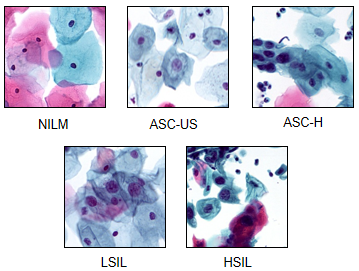
\includegraphics[scale=0.8]{figures/tbs.png}
    \caption{Examples of cervical cells in different degrees: NILM is the ``normal'' case, while the rest are abnormal types, and ASC-H, LSIL and HSIL are the advanced abnormal types indicating a more severe progression of symptoms.}
    \label{fig:tbs}
\end{figure}


Conventional TCT examinations are implemented by visual inspection of the stained samples with collected cervical cells under the microscope, which requires substantial expertise from pathologists and becomes a challenging problem worldwide. It can be observed from Fig. \ref{fig:tbs} that the differentiation of different cervical cell types is subtle in appearance and morphometry. And pathologists rely on key (abnormal) cells to make diagnoses. Especially in the low-middle income areas where healthcare resources are limited, the screening needs are relatively more challenging for pathologists to handle. Therefore, a fully automatic computer-aided diagnosis (CAD) system is highly desired for TCT screening, which is implemented based on the scanned whole-slide images (WSIs) and completes the screening in a high-throughput and robust way.




Recently, deep learning has emerged as a promising tool for the automatic diagnosis of many diseases. 
In the field of pathology, the screening of cervical abnormalities has drawn a lot of attention. Due to the image size of the scanned WSIs which are generally huge (e.g. normally about $30000\times 40000$ in image size for a WSI sample under study), the CAD system for WSI screening is usually implemented in a hierarchical manner. 



% Generally speaking, concerning the complexity of the screening task, deep learning methods usually solve this problem step by step. 
For example, Zhou et al. \cite{zhou2021hierarchical} proposed a three-step framework for TCT screening.
First, a cell detection network is trained to localize the suspicious abnormal cervical cells from WSI.
Then, the patch is center-cropped for each suspicious cell, and further processed through a classification model to tell whether the patch is positive or negative. 
Finally, the typical positive patches determined by the patch-level classification are further ensembled, such that the overall positive/negative diagnosis is produced for the WSI at the sample level. 

Similar ideas are also shared by several related works in the literature.
Cao et al. \cite{cao2021novel} proposed the cell detection model of AttFPN, which benefited from the clinical knowledge and the attention mechanism, to improve the detection performance. Cheng et al.
\cite{cheng2021robust} proposed a progressive identification method that combined multi-scale visual cues to identify abnormal cells, and a recurrent neural network (RNN) was adopted to complete the sample-level classification based on the patches cropped from the abnormal cells. Wei et al. \cite{wei2021efficient} proposed the cervical screening method which focused on improving both the cell detection network and the classification network. They adopted the YOLO architecture and added a variety of convolution kernels of different sizes to adapt to the highly diverse cell clusters, and they also used the transformer to improve classification performance.


% \todo{What is the limitation of existing methods or the challenge unresolved yet? You need summarize the problems first, then propose your method solve the problems.}

Although many works have contributed to TCT screening, there are still several challenges that remain unsolved: 

\begin{itemize}
    \item 
   The differentiation of cervical cells in TCT examinations is challenging even for professional pathologists. 
   And the classification is quite subjective although the TBS specifications illustrate the cervical cell abnormality in different types. There are unavoidable cell sets that cannot be easily recognized by the pathologists, which are recognized as the \textit{hard} samples in our work\todo{I don't think it's correct here. We didn't use pathologist labeling to identify hard samples}. As the \textit{ground-truth} labels of those cells are not fully convincing, they need to be handled in a specific manner when constructing the learning-based classifiers.
    \item 
    As the CAD-based TCT examinations are generally implemented in a hierarchical manner, the WSI-level classification needs to be implemented based on the aggregation of the detected suspicious cell results. The ensembling strategy needs to be spatially dynamic, as individual cells from different locations may have evidence of varying strength to support the sample-level decision.
    \item 
    Finally, the screening system should be highly sensitive overall, such that false negatives can be mostly suppressed and cervical abnormality can raise alert as early as possible. 
    Therefore, the sample-level decision is usually ensembled from a relatively large number of cell patches per WSI (e.g., 20 in our implementation), in case the cell detection may not identify those positive cells if the number is too small \cite{zhou2021hierarchical}. 
    Contrarily, those patches often have similar appearances. And even for a positive sample, the to-be-ensembled patches may have appearances that are close to negative. Thus, one may need to pay special attention to suppressing the redundant and distorting patches when ensembling them.
\end{itemize}


To solve the problems above, here we propose a novel TCT screening framework that effectively combines traditional convolutional neural network (CNN) and transformer structure, aiming at improving the sample-level classification performance through the powerful local feature extraction capability of CNN, and the global feature fusion capability of the transformer structure. We also propose a novel clustering loss\todo{Still clustering loss?} to improve the capacity of feature representation for our patch-level CNN model. For sample-level classification, we propose a novel score embedding and hierarchical token aggregation strategy to deal with different patches within the sample. The main contributions of our work are listed as follows:  




\begin{itemize}
    \item We design a novel TCT screening framework, which combines CNN and transformer to further fuse global features on the basis of effectively extracted local features, 
    and improve classification on sample-level for cervical cancer screening.
    \item We design a novel patch-level image feature extraction strategy from the CNN network, using the hard patches mining method to make the feature space more compact and reasonable. Thus, the model can have a stronger ability to distinguish hard patches.
    \item We design the classification scores for each patch and treat these scores as unique location information in the feature space to have a score embedding for each patch, thus allowing the transformer model to better exploit the relationship between different patches.
    \item We develop a novel token pooling strategy with the tokens input into the transformer to simplify more representative tokens, so that the network can learn which tokens to pay attention to, and ultimately improve the classification effect.
\end{itemize}

The rest of this paper is organized as follows, Section \ref{sec:related} is the related works, which contains the common structures in medical images and the common methods for feature-based learning. Then in Section \ref{sec:method} we introduce our proposed method, which mainly consists of the patch-level classification model and the sample-level classification model. In Section \ref{sec:experiments} we conduct experiments to both evaluate the effectiveness on the patch-level and sample-level, and finally the related discussions and conclusions presented in Section \ref{sec:discussion} and Section \ref{sec:conclusion}, respectively.





\section{Related Works}\label{sec:related}
In this section, we first explore the current development and applications of deep learning in the field of cervical cancer screening, which generally includes detection, segmentation and classification tasks. Then, we present a comprehensive investigation of representation learning and its applications in the field of pathology screening. 

\subsection{Cervical Cancer Screening using Deep Learning}
With the development of deep learning technology, many attempts have been made in automatic cervical cancer screening for resolving the issues of labor-intensive and subjective judgments from the manual screening by pathologists. Generally, all these researches can be divided into two major categories: 1) the detection and segmentation of cervical cells from the WSI, and 2) the classification to aggregate visual features from the cervical cell sets for determining their abnormality. A large number of efforts have been made in the cell-level detection and segmentation tasks, since it is a prerequisite to find suspicious cells from WSIs before further analysis. For example, Zhao et al.\cite{zhao2019automated} developed the Deformable Multipath Ensemble Model (D-MEM) aiming at cervical cell nuclear segmentation, and Zhang et al.\cite{zhang2019binary} further proposed a binary-tree structured cervical cell nuclear segmentation network which incorporates attention mechanisms for improvements of segmentation performance. Zhou et al. ~\cite{zhou2021hierarchical} investigated the current widely-applied detection models including Faster-RCNN\cite{ren2015faster}, YOLO\cite{redmon2018yolov3}, RetinaNet\cite{lin2017focal} and etc., and demonstrated in experiments that RetinaNet has the advantages of both high accuracy and efficiency compared with alternatives in the applications of detecting abnormal cervical cells in WSI. Du et al. \cite{du2021false} proposed a semi-supervised learning method with attention guidance for false positive suppression of cervical cell abnormality detection task.  

On the other hand, the classification task has also played an essential role in the cervical cancer screening pipeline, where it is applied to further refining and determining if the selected cells have abnormality. The corresponding classification methods can be designed either for the cell-level or patch-level which targeting on single cells, or for the image-level or sample-level which focuses more on summarizing the overall screening results from the cervical cell sets under study. Nowadays with the developments of deep learning the classification approaches have become much more advanced with high accuracy and robustness than ever before. Generally, in natural images the classification model is constructed by using the pre-train model as backbone, which can help improve the stability of model training and guarantee the representation capacity of the extracted deep visual features. The most widely-applied pre-train models are VGG and ResNet\cite{bizzego2019evaluating}, and with different configurations such as layer numbers for fitting with various application scenarios. Recently, transformer\cite{vaswani2017attention} technology has drawn attention in the field of deep learning, which is developed based on the self-attention mechanism and has demonstrated its representation ability in the classification tasks. Further extension of transformer has been made in the computer vision domain, and Vision Transformer (ViT) method was proposed by Dosovitskiy et al. \cite{dosovitskiy2020image} which has shown excellent performance on a wide range of visual tasks\cite{xu2022groupvit}, \cite{liu2022cvm}. 
% Add some current developments of classification methods in the computer vision field

Many attempts have also been made in cervical cancer screening using deep learning technology. For example, Zhang et al.\cite{zhang2019binary} developed DeepPap software which implements cell-level classification using convolutional neural network (CNN), and Taha et al.\cite{taha2017classification} proposed the cell-level classification method by firstly using a pre-trained CNN model for feature extraction and then SVM for classification. As for the sample-level classification, Zhou et al. ~\cite{zhou2021hierarchical} proposed a hierarchical framework that progressively gauges the visual features from the detected suspicious cells for the final determination of the WSI screening. However, all the above-mentioned classification methods are implemented by simply ensembling the extracted visual features from the detected cell patches and feeding them into the classification model, without considering the feature status of these patches in the feature space, and therefore cannot conduct comprehensive aggregation of these patch information and undermines the performance of the classification tasks. 

\subsection{Representation Learning and Classification}
With the development of deep learning, the architecture of the constructed model has become increasingly large and complex, and many extracted features from the deep learning models are actually abundant, which undermines its capacity to characterize the target images and achieve classification models with high accuracy. In this way, representation learning has been intensively investigated to solve the above-mentioned issue and further optimize the deep learning model \cite{bengio2013representation}. Generally, representation learning aims at automatically extracting and optimizing the features in a more systematic manner, and can be categorized as supervised, unsupervised and self-supervised learning depending on how we utilize the data labels in the model training. 

Many representation learning methods are developed aiming at finding the optimal features under the given scenarios and machine learning tasks. For example, Weng et al. \cite{weng2019multimodal} used the representation learning method of corresponding feature constraints between different modal images to successfully enable the model to complete multi-task under multi-mode. Moriya et al. \cite{moriya2018unsupervised}used similar clustering methods to aggregate features to achieve better feature representation, so as to provide more precise and accurate features for model segmentation tasks. Besides, there are also many representational learning methods designed for different model characteristics, Liu et al. \cite{liu2021swin} and Rao et al. \cite{rao2021dynamicvit} used the strategy of representation learning in ViT\cite{dosovitskiy2020image}, Adnan et al. \cite{adnan2020representation} used the strategy of representation learning in GCN, which have improved the feature expression efficiency of the models. 
 
Some efforts have also been specifically made in the field of pathology image classification. For example, Boyd et al.\cite{boyd2021self} and Pati et al. \cite{pati2021reducing} used representation learning to add an extra loss on features to help the model do better self-supervised learning with digital pathology. In this paper, we adopt the method of representation learning on the classification models of both patch level and sample level, and independently designed different strategies aiming at improving the feature expression ability of the models, and with experiments to show its effectiveness and robustness.

\section{Method}\label{sec:method}

% \subsection{Pipeline for Automatic TCT Screening}
% \label{section-3-1}
The overall TCT screening framework is presented in Fig. \ref{fig:overview}, which consists of three major steps in a hierarchical manner: 

\begin{figure*}[ht]
    \centering  
    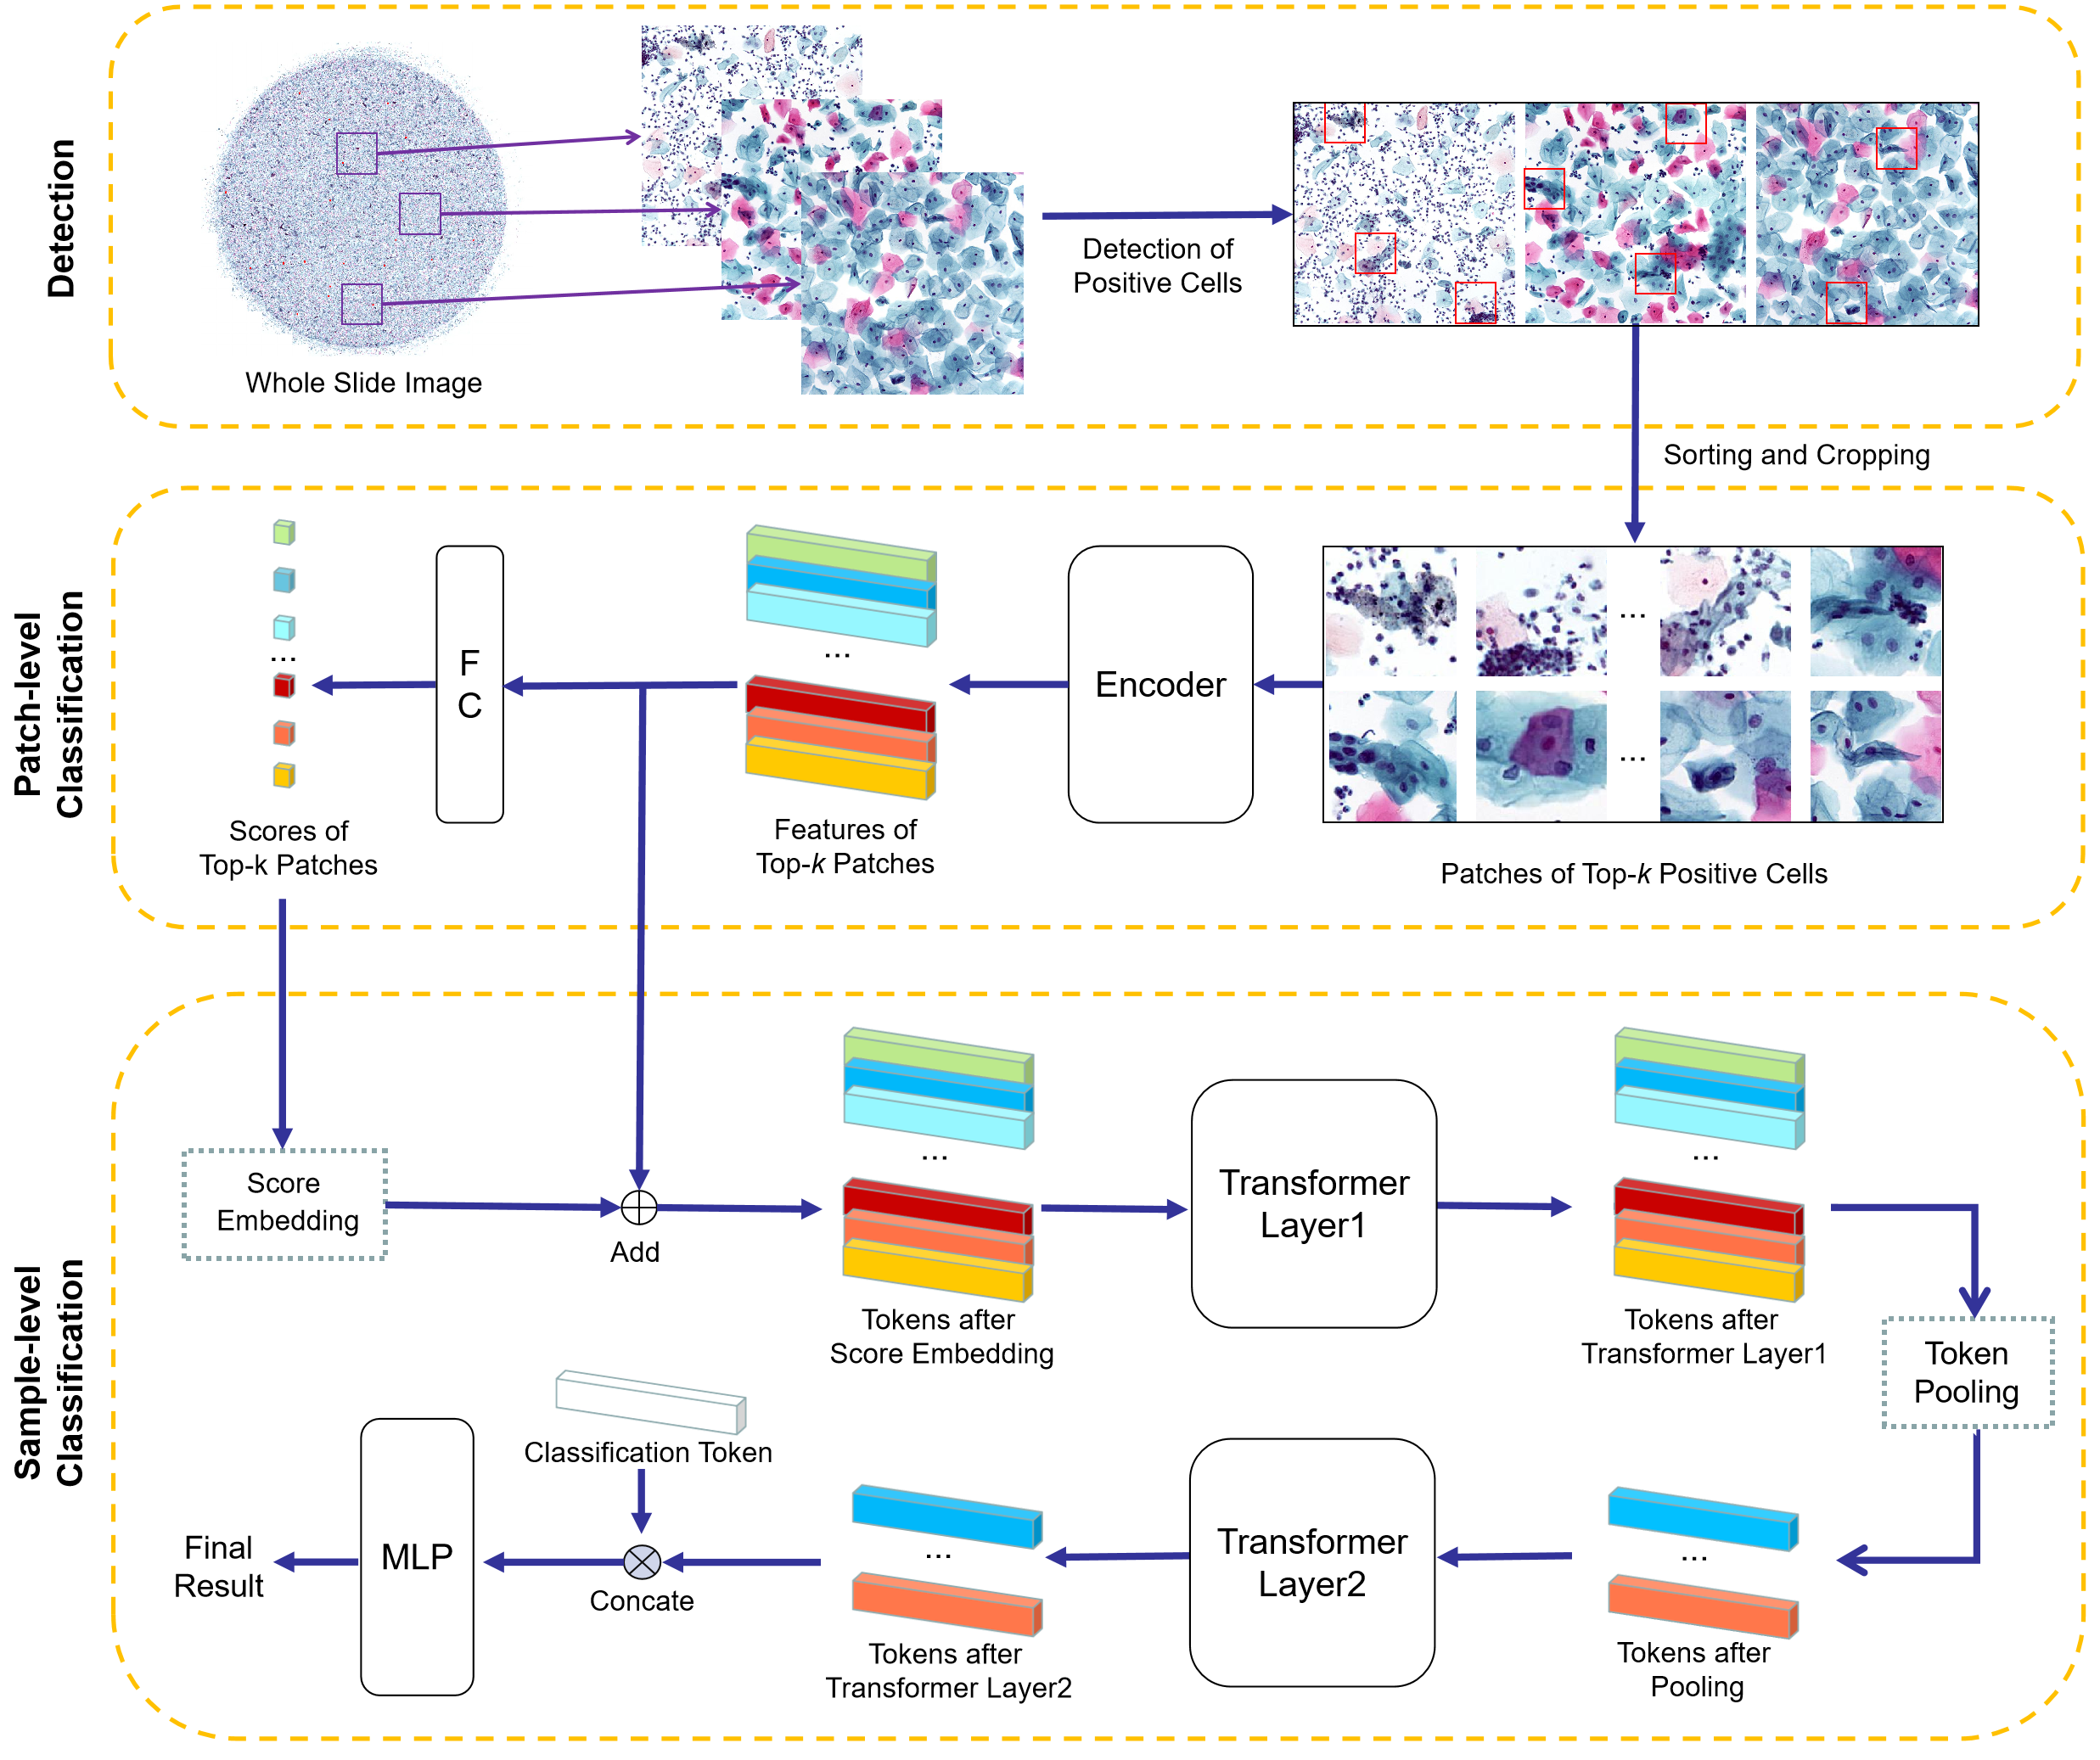
\includegraphics[width=\textwidth]{figures/pipeline.png}
    \caption{The overall pipeline of TCT screening, including the detection, patch-level classification and sample-level classification steps. The detection step intends to locate suspicious cervical cells, and extract their corresponding patches with the size of 224$\times$224. The patch-level classification step obtains the features and scores of the top $k$ patches with the highest possibility of abnormality, which are fed into score embedding and token pooling in transformer layers, and then concatenated with the classification token for passing through MLP to get the final result in the sample-level step.}
    \label{fig:overview}
\end{figure*}

\begin{itemize}
    \item 
    \textbf{Step 1:} We acquire the WSI data for each sample and conduct necessary quality control as well as pre-processing works. 
    Then, we apply an in-house cell detection network and identify those cells that are suspiciously positive (e.g., highlighted by red boxes \todo{They are not red enough in the figure} in the top row of Fig. \ref{fig:overview}). To ensure the feasibility of the detection process, every WSI sample is partitioned into a collection of tiled images sized 1024$\times$1024, which are used for suspicious cell detection separately. 
    % Besides, since the screening aims to pick up all samples that are eventually diagnosed as positive, the cell detection here usually works at high sensitivity, leading to many false positives in the detection outcomes from a very large WSI sample. 
    % Therefore, for each detected cell, we will perform patch-level classification in the second step to refine the detection result.
    \item 
    \textbf{Step 2:}  For each detected suspicious cell, we center-crop its corresponding patch (224$\times$224) to collect a patch-level cervical cell dataset. The patches in the dataset have been manually labeled by the pathologists and are used to train a binary classifier. Our aim is to use the classifier for false-negative suppression of the detected cells, which are also ranked based on the confidence score from the classifier. Here the top-$k$ (=20 in our implementation) cells with the highest scores are selected for the final sample-level diagnosis in Step 3. 
    \item 
    \textbf{Step 3:} We ensemble all top-$k$ patches via a transformer network to attain the sample-level classification. Particularly, we use the feature embedding from the patch-level classifier as the token for each cell patch, which is fed into the transformer. The transformer network is applied here to determine the contributions of individual patches dynamically, and group the tokens according to the intrinsic similarity among the patches. In this way, the feature representation after pooling becomes more effective to characterize the abnormality status of the WSI sample, leading to a more accurate sample-level diagnosis.
\end{itemize}

Note that our TCT screening system is not designed to depend on the specific detection method, and we also explore its feasibility by evaluating the effectiveness of three widely-applied detection models adopted in the pipeline, which are RetinaNet, FasterRCNN and Yolov3. Section \ref{section-3-2} and Section \ref{section-3-3} further illustrate the implementation details of the patch-level and sample-level classification steps, respectively.


\subsection{Patch-Level Classification}
\label{section-3-2}

% The patch-level classification deals with the patches centered on the suspicious cells that are previously detected. Since the cell detection is designed to be highly sensitive to avoid missing the potentially positive cells, the patch-level classification here is necessary to reduce the false positives in the detection results. 

% In order to make model have better feature representation and classification ability, we impose additional feature clustering constraints on the model based on the cross-entropy loss function. Furthermore, unlike the normal direct clustering constraint on each class, we take a selective cluster constraint on those patches which are a part of one batch. The process of different losses is shown in Figure \ref{fig:patch}.

We illustrate patch-level classification in Fig. \ref{fig:patch}.
Particularly, we use SEResNext50 as the backbone for the encoder. 
Individual patches pass through the convolutional layers, pooling layers, and a global average pooling (GAP) layer, to reach a 2048-dimensional feature space. 
The feature vector of each patch is further processed by a fully connected (FC) layer to yield the classification result. The classification network is further optimized by the cross-entropy-loss. 

\begin{figure*}[ht]
    \centering
    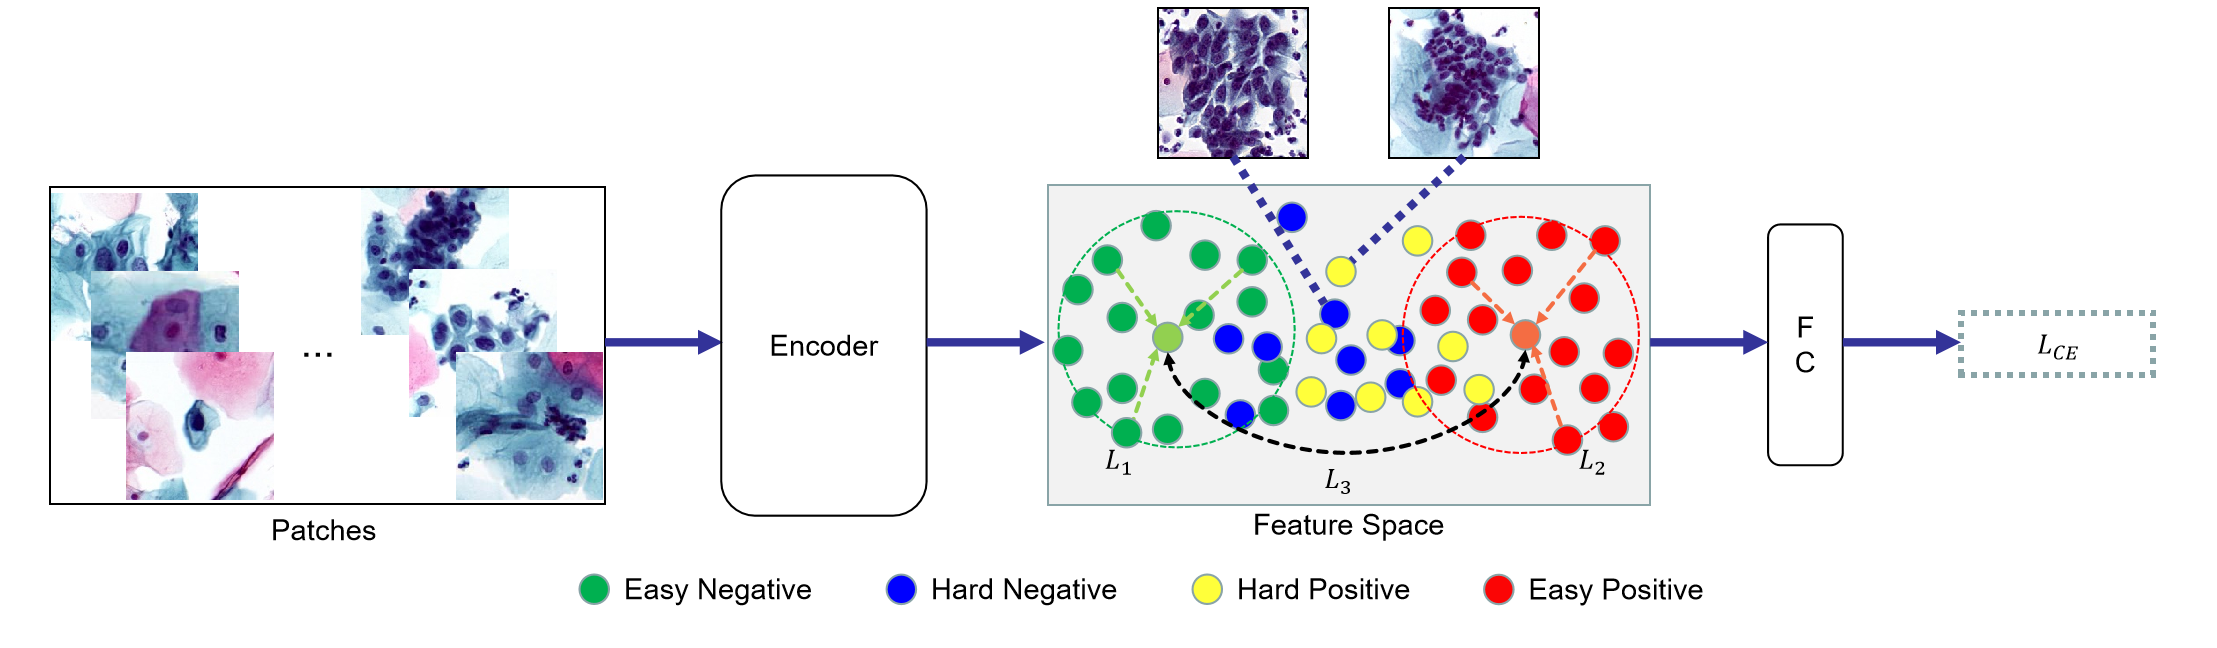
\includegraphics[width=\textwidth]{figures/patch-level.png}
    \caption{Diagram of our hard patch mining method on patch-level classification, the green points represent the features of easy negative patches(EN), blue points represent the features of hard negative patches(HN), yellow points represent the features of hard positive patches(HP), red points represent the features of easy positive patches(EP). Up of the feature space are two examples of HN and HP with similar appearance, of which left are normal cells, and the changes in cell morphology may be related to micro-adenogenesis, which is common in the late menstrual cycle of women taking oral contraceptives, and right are typical positive cells. We impose constraints on EN and EP which is ${L}_{1}$ and ${L}_{2}$ to make them closer to their respective cluster centers, and ${L}_{3}$ make features between different classes far away.}
    \label{fig:patch}
\end{figure*}
% However, as neglected by many conventional methods, the confusion about this classification task mostly originates from the hard patches, while the relatively easy patches can be well handled.
% Therefore, our patch-level classification model will emphasize the roles of those hard patches by referring to the data distribution in the latent feature space. 


It is non-trivial to tag a certain patch as positive or negative. 
There are hard patches, the labels of which have high uncertainty even for professional pathologists, which are shown in Fig. \ref{fig:patch}. 
In binary classification, simply calculating the cross-entropy loss cannot effectively separate those hard-positive and hard-negative patches. \todo{The motivations of why making these two extra labels unremain unclear to me.}
Therefore, we impose an additional constraint of hard-patch mining in patch-level classification.
With hard-patch mining, the easy-positive and easy-negative patches are pushed apart after they are embedded in the latent space. 
The hard samples can utilize the wide gap between the easy-positive and easy-negative patches for their distributions in the latent space.
In this way, our patch-level classification network is capable of better modeling the latent feature space, and distinguishing the positive/negative patches.

The hard patches are identified according to their contributions to computing the cross-entropy loss as in Fig. \ref{fig:patch}. 
In particular, we divide one batch of patches according to a certain threshold $m$ \todo{where is this $m$ coming from?} of the CE loss value of every patch in this batch (which we test with 0.3, 0.4, 0.5, 0.6, 0.7 in our experiment, and finally defined as 0.5 in our method), and divide them into easy patches (the loss value smaller than m) and hard patches (the loss value bigger than m).

We encourage the easy-negative and easy-positive to distribute compactly. 
To this end, we calculate the mean feature vectors for the easy-negative and easy-positive patches based on their feature embedding in the previous epoch. 
We denote the two mean feature vectors as $\bar{x}^e_{n}$ and $\bar{x}^e_{p}$, respectively.
Next, we calculate the cosine similarity between each patch in the current batch and the corresponding mean feature vector, which is a commonly used metric to measure the similarity between two vectors ~\cite{nguyen2010cosine}, \cite{zhang2022whole}, \cite{cao2022parallel}. Within the two groups of easy-positive and easy-negative, we define two losses:
\begin{equation}
    \begin{aligned}
        L_{1}&=1-\frac{1}{|\mathcal{B}^e_{n}|}\sum_{i \in {\mathcal{B}^e_{n}}}  S( x_{i},\bar{x}^e_{n} ).\\
        L_{2}&=1-\frac{1}{|\mathcal{B}^e_{p}|}\sum_{i \in {\mathcal{B}^e_{p}}}  S( x_{i},\bar{x}^e_{p} ).
    \end{aligned}
\end{equation}
Here, $\mathcal{B}^e_{n}$ and $\mathcal{B}^e_{p}$ indicate the current batches of the two groups of easy-positive and easy-negative. 
And the two losses encourage all easy patches to distribute compactly within their groups, implying more space is left for the hard patches in the latent space.
We further separate the EN and EP classes by introducing $L_{3}=S(\bar{x}^e_{n},\bar{x}^e_{p})$. In this way, the two classes can move apart from each other in the latent space.
\begin{figure*}[ht]
    \centering
    \includegraphics[scale=0.2]{figures/token.png}
    \caption{The similarity maps of the tokens, We selected three typical samples, namely, NILM, ASC-US and High-Level samples, the top 20 patches obtained from the detection network are as shown in the figure. The corresponding value of each patch is their score after passing through the patch-level classification network. The similarity map of the feature vectors obtained by encoding the 20 patches is on the right.}
    \label{fig:vit}
\end{figure*}
Finally, we derive the overall clustering loss:
\begin{equation}
L_{p}=L_{ce}+L_{1} + L_{2} + L_{3}.
\end{equation}
The first term $L_{ce}$ is the cross-entropy loss for the classification. And the rest three terms ($L_{1}$, $L_{2}$, $L_{3}$) are for the hard-mining loss.
In this way, we expect the intra-class feature encoding of the easy patches to be relatively similar, while the inter-class feature encoding should be far away. 
With the constraint encoding of the easy patch feature vector, the feature encoding of the hard patch will also gradually be different, which will increase the feature space encoding ability of the patch-level classification model.




%In order to enhance the interpretability of our method, we visualize the token correlation, and we select three typical samples, NILM, ASC-US and a high-level, which NILM is the negative sample and ASC-US, high-level is the positive sample. The first column shows the original pictures of one sample, which consists of 20 patches, and each patch is 224*224 in size. The second column shows the correlation between 20 tokens, these tokens have obvious characteristics of aggregation, which means that if we directly use 20 tokens for operation, a lot of redundant information will be generated, and there are not always only two types of clusters, so an arbitrary number of cluster centers The clustering algorithm is necessary. The third and fourth columns show the importance of the classification token. As shown in the figure, the token that contributes more to the classification token has a darker color. The visualization results show that our method can effectively integrate the key The token is extracted from a bunch of tokens.

\subsection{Sample-level Classification}
\label{section-3-3}

The sample-level classification relies on the top-\textit{k} suspicious patches, which is illustrated at the bottom of Fig. \ref{fig:overview}. 
We input the top-\textit{k} patches into the transformer network. 
Specifically, we use the feature vector in the latent space before the FC layer of the patch-level classifier as the token of each input patch.
The network has two transformer layers, the input dimensions of both transformer layers are 2048, and their depths are 8 and 4 respectively. 
% Since there are often some patches in multiple patches whose feature expressions are very similar, the transformer network structure needs to integrate the feature information of the top k to further extract the global feature information from them, and finally get a classification result of the whole sample. 

% The patch-level classification provides scores, rather than only binary outcomes, to allow us to rank the patches according to their likelihood of being positive. 
% Specifically, we pick up the top-\textit{k} patches, and feed them to the transformer based on their latent representation extracted by the patch-level classification network. 
% The transformer architecture can integrate those \textit{k} patches and reach a global representation of the whole WSI.

Particularly, In order to better transfer the independent information of each patch to the model, similar to position embedding in Vision in Transformer (ViT)\cite{dosovitskiy2020image}, we propose score embedding to input the score of each patch in the patch level classification model into the transformer layer. Next, according to our observation in Fig. \ref{fig:vit}, many features of different patches are redundant, so we used the token pooling strategy to help the model filter redundant feature expressions. The specific methods of score embedding and token pooling are as follows.



\subsubsection{Score Embedding}
Preserving the independent information of each part of a whole has been proven to be an effective method in the field of deep learning, such as patch position embedding in an image\cite{dosovitskiy2020image}, word position embedding in language text\cite{vaswani2017attention}, and graph embedding in recommendation system\cite{goyal2018graph}, 
The abnormality can occur in anywhere of the WSI. 
How to effectively embed information on cells in different patches of images so that the model can make full use of this information and make different patches have independent information expression will become a problem to be solved\todo{I don't understand this sentence. What is independent information?}. Although WSI images, like those in vit, are divided into many small patches, since WSI images are processed after uniform centrifugation, the location information of each patch is no longer meaningful. So we use score embedding instead of position embedding to solve this problem.



We choose the classification score obtained by using the feature vector of each patch through the fully connected layer of the classification model at the patch level as the location information of the feature space for feature space location embedding, which is shown in Figure\ref{fig:overview}. 
We expand these scores to the same shape as features on the channel dimension, which is 2048 dimensions, and add them to the original features to get a new set of features.
This strategy is very simple but effective. It can maintain the independent information of each patch image when the location information cannot be used, so as to improve the classification accuracy.


\subsubsection{Token Pooling}
To observe whether the features input to the transformer layer is valid, we calculate the similarity map for all features of the top k patches of a sample. As shown in the figure\ref{fig:vit}, we sort each patch from small to large according to its classification score. The similarity map also follows this sort. It can be seen that in some samples, such as a) NILM, many patch features have strong similarities. In addition, among the top k patches of different samples, the degree of similarity of tokens is also different. The k pictures of negative samples tend to have similar features, while the k pictures of positive samples show a group-by-group approach, but the number of groups is often uncertain.
So in order to use tokens more concisely and efficiently, we use the token pooling method to reduce redundant tokens to highlight important tokens, so that the model can better adapt to the task of negative and positive classification.


Due to the uncertainty of the number of groupings, we generally refer to the affinity promotion (AP)\cite{frey2007clustering} algorithm to perform the token pooling operation. The AP algorithm updates the attractiveness and attribution information of each point in the similarity matrix, and adds the attractiveness and attribution after reaching the preset number of iterations to obtain the cluster center. Specifically, in our proposed method, after obtaining the features after score embedding, we first use a transformer layer to calculate the self-attributes of these features. After obtaining a group of new features, we use the AP algorithm to cluster these features. After obtaining n-class features, we perform average pooling operations on these n-class features to obtain more concise feature expression after aggregation.


In addition, since we need to unify the number of tokens in the same batch, we use a small trick, which will find the sample with the largest number of tokens in the current batch, and align the tokens of other samples with it by filling zero with it. 

Later, we again calculate the self-attention of these simplified features through another transformer layer, and splice a learnable classification token with it. Finally, the final classification result is obtained after the MLP module.


\begin{table*}[ht]
    \setlength\tabcolsep{5pt}
    \centering
    \caption{Results on patch-level classification of different methods. }
    
        \begin{tabular}{|c|c|c|c|c|c|c|c|c|c|c|c|c|c|c|c|}
        \hline
        
        Backbone& \multicolumn{5}{|c|}{ResNet50} & \multicolumn{5}{|c|}{ResNext50}& \multicolumn{5}{|c|}{SEResNext50}\\
        \hline
        % \diagbox{Backbone}{Metric} %添加斜线表头
            Metric ($\%$)    & ACC&AUC &Precision&Recall&F1 Score&  ACC&AUC &Precision&Recall&F1 Score& ACC&AUC &Precision&Recall&F1 Score\\
        \hline
        $L_{ce}$       & 77.76 & 79.66&  73.12&77.94  &75.45&78.94 &80.16& 76.15&73.26 &74.68 & 79.33&81.45&74.44&78.57&76.45\\
        \hline
        Ours (p=0.3)       & 78.59  & 81.77 & 73.08&79.67 &76.23  &79.31& 82.03 &74.82&77.93 &76.34 &80.55 &83.34 &75.77 &84.87  &80.06\\
        \hline
        Ours (p=0.4)     & 80.63& 82.57  &75.34&81.76 & 78.42&80.32  &82.77  &75.58&78.83 & 77.17&81.44 &83.96 &77.87 &82.85  &80.25\\
        \hline
        Ours (p=0.5)     &82.28 & 84.43  &78.12&83.33 &80.64& 82.87 & 84.32  &79.12&81.07 & 80.08&83.56 &85.39 & 79.04&83.73  &81.32\\
        \hline
        Ours (p=0.6)    & 81.64& 83.54  &77.37&79.54 &78.44&82.33  &83.85  &78.80&80.13 & 79.46&82.53 &84.46 &76.35 &82.41  &79.26\\
        \hline
        Ours (p=0.7)   &79.59 & 81.97  &76.55& 78.46&77.49&80.17  &82.18  &75.78&78.33 & 77.03&81.13 &82.83 &76.74 &81.93  &79.25\\
        \hline
        
        \end{tabular}
        
        \label{tab:patch-results}
    \end{table*}
\begin{table*}[ht]
    \setlength\tabcolsep{5pt}
    \centering
    \caption{Results on sample-level classification of different methods.}
        \begin{tabular}{|c|c|c|c|c|c|c|}
        \hline
        \diagbox{Method}{Metric ($\%$)}& ACC &  AUC&Recall&Precision&F1 Score\\
        \hline
        Average Pooling (AVG) \cite{cao2021novel}       & $76.82\pm0.75$ & $84.32\pm1.07$& $73.49\pm0.99$& $78.62\pm1.20$& $75.96\pm0.84$\\
        \hline
        Support Vector Machine (SVM) \cite{zhou2021hierarchical}       & $76.82\pm0.75$ & $84.32\pm1.07$& $73.49\pm0.99$& $78.62\pm1.20$& $75.96\pm0.84$\\
        \hline
        Multilayer Perceptron (MLP) \cite{zhou2021hierarchical}       & $78.70\pm1.94$ & $85.60\pm0.63$& $60.78\pm4.11$& $84.52\pm1.08$& $73.90\pm3.11$\\
        \hline
        Recurrent Neural Network (RNN) \cite{cheng2021robust}       & $80.89\pm1.29$ & $87.17\pm1.42$& $73.71\pm2.52$& $84.08\pm2.77$& $79.82\pm0.96$\\
        \hline
        Graph Attention Network (GAT) \cite{zhang2022whole}       & $85.79\pm1.21$ & $92.52\pm0.91$& $82.63\pm2.04$& $88.15\pm1.39$& $85.28\pm1.27$\\
        \hline
        Ours       & $89.51\pm1.57$ & $93.79\pm0.95$& $88.65\pm1.72$& $91.13\pm1.41$& $89.87\pm1.19$\\
        \hline
        
        \end{tabular}
        
        \label{tab:sample-results}
    \end{table*}

\section{Experimental Result}\label{sec:experiments}
Our experiments are four-fold. First, we conduct experiments on different network backbones to compare the original patch-level classification method and our proposed classification method with clustering constraints to prove its effectiveness. Second, we compare our sample-level classification method with state-of-the-art methods (such as Graph Attention Network) to verify the effectiveness of the transformer structure combined with CNN. Third, we conduct ablation study on each component of the proposed method to independently verify the effectiveness of each component. Finally, we combine different detection network modules to verify the universality of our method.\par
In Section \ref{section-4-1}, We first introduced the data set we used and the relevant experimental settings, in Section\ref{section-4-2}, We introduced the results of the patch-level classification experiment, and in Section\ref{section-4-3}, We introduced the results of sample-level classification experiment, which includes three parts: comparison with SOTA results, ablation experiment and universality experiment related to detection model.


\subsection{Datasets and Experimental Setting}\label{section-4-1}
We have considered two tasks of patch-level and sample-level classification in this work. 
Therefore, there are two datasets to validate our method. 
\begin{itemize}
    \item 
    The first patch-level dataset consists of 25,143 patches (negative: 13,264; positive: 11,879), each of which is cropped to the size of 224$\times$224. 
    Given this dataset, we divide the training and test ratio as 4:1, and aim to verify the performance of the proposed patch-level classification.
    \item 
    The second sample-level dataset consists of 6,947 samples (negative: 3,485; positive: 3,462). 
    For each WSI contributed from a certain sample, we apply an in-house detection tool to pick up 20 patches that are most likely to be positive~\cite{zhou2021hierarchical}. 
    We aim to combine the proposed patch-level and sample-level classification to complete the screening based on the detected patches of the samples. 
    Similarly, we also divide the training set and test set according to the ratio of 4:1.
\end{itemize}   
  
Note that the samples contributing to the second dataset are not involved in the first dataset; thus the two datasets are fully independent. 
A professional pathologist with 13 years of experience has conducted the patch-level and the sample-level diagnoses, providing us the ground-truth labels according to the TBS guideline. 

For patch-level classification, we examine the performance of our method with three different backbones including ResNet50, ResNext50 and SEResNext50, which are all common choices for classifying histopathology images. We have trained our networks by using data augmentation on color with the Adam optimizer. The initial learning rate is 1e-3, the learning rate decay factor is 0.95, and the batch size is 64.
For subsequent sample-level classification, we adopt two transformer layers with depths equal to 8 and 4, score embedding block, normalization layers and a MLP to construct the model, the initial learning rate is 1e-4, batch size is 8, and we use cosine annealing schedule to adjust the learning rate.
For all classification experiments, we use ACC, AUC, precision, recall and F1 score as the metrics, and our networks are all pre-trained on ImageNet. 




\subsection{Patch-Level Classification}\label{section-4-2}

For patch-level classification, we set different p values (0.3, 0.4, 0.5, 0.6, 0.7) as the thershold between easy patches and hard patches to compare with the case which is only constraint by cross entropy loss. And for comprehensive comparisons, we adopt three different classification backbones, each of which is widely applied in pathology images. The comparison is shown in Table \ref{tab:patch-results}.



We evaluate our method with different backbones and with different loss combinations. 
The classification performance of AUC, precision, recall, and F1 score is reported Table \ref{tab:patch-results}.


One can observe from the table that, our patch-level baseline, which is trained with vanilla cross-entropy loss function, got 79.66\% AUC on ResNet50 model, 81.77\% AUC on ResNext50 model, 84.57\% AUC on SEResNext50 model, to contrast, the model trained with both cross-entropy loss and hard patch mining loss got higher AUC scores than the baseline with all settled p values. Particularly, when we compare with different p values among our hard patch mining strategy, we can find that the results of p values settled to 0.5 are the best results, which shows the importance of threshold to distinguish between easy patches and hard patches. Too large or too small threshold can not accurately reflect the distribution of hard and easy patches in the dataset. A good threshold can make the model adapt to the accurate distribution of the dataset more quickly, thus improving the characteristic coding ability of hard patches. 
\par





\subsection{Sample-Level Classification}\label{section-4-3}
\subsubsection{Comparisons to State-of-the-Art}

We compare with the related works of deep learning based cervical cancer screening methods, the results on the sample-level is shown in Table \ref{tab:sample-results}. We can observe that the methods of connecting patches among samples (such as RNN and GAT) can have a better performance than those methods that simply process each patch to get the final classification results (such as SVM and MLP), which once again illustrates the importance of linking patches together. However, our transformer based method has achieved the best results. On the one hand, it has stronger global connectivity and integrates all patch information. On the other hand, the token pooling operation in our method has further obtained more concise but effective information, which will also be proved in the following ablation experiments.
In general, the above results proves that the combination of transformer structure and CNN structure is effective in sample level classification, and have a significant improvement compared with other methods.

\begin{table*}[ht]
\centering
\caption{Ablation study.}
{
\begin{tabular}{|c|c|c|c|c|c|c|c|c|}
\hline
\multicolumn{4}{|c|}{Method} & \multicolumn{5}{|c|}{Metric ($\%$)}\\
    \hline
Hard Patch Mining&\multicolumn{2}{|c|}{Token Pooling}&Score Embedding&ACC&AUC&Recall&Precision&F1 Score\\
\hline
 &\multicolumn{2}{|c|}{\XSolidBrush}&& $83.37\pm1.01$ & $87.97\pm0.69$& $78.83\pm1.09$& $86.13\pm1.22$& $82.36\pm0.88$\\
 \hline
 & \multicolumn{2}{|c|}{K-means}&&         $85.74\pm1.17$ & $91.97\pm0.75$& $83.99\pm0.96$& $87.87\pm1.31$& $85.89\pm1.07$\\
 \hline
 &\multicolumn{2}{|c|}{AP}&&     $86.32\pm1.38$ & $92.24\pm1.23$& $84.55\pm1.37$& $86.67\pm1.28$& $85.60\pm1.11$\\
 \hline
 \ding{52} &\multicolumn{2}{|c|}{\XSolidBrush}&&     $84.59\pm1.32$ & $89.53\pm1.14$& $81.11\pm1.53$& $86.07\pm1.36$& $83.52\pm1.09$\\
 \hline
  \ding{52}& \multicolumn{2}{|c|}{K-means}&&       $88.77\pm0.99$ & $93.33\pm1.15$& $85.57\pm1.32$& $92.44\pm1.03$& $88.87\pm0.75$\\
 \hline
  \ding{52}&\multicolumn{2}{|c|}{AP} &&      $88.19\pm1.35$ & $92.88\pm1.25$& $85.31\pm1.54$& $90.97\pm1.33$& $88.05\pm1.14$\\
\hline

 &\multicolumn{2}{|c|}{\XSolidBrush}&\ding{52}&  $83.37\pm1.01$ & $87.97\pm0.69$& $78.83\pm1.09$& $86.13\pm1.22$& $82.36\pm0.88$\\
 \hline
 &\multicolumn{2}{|c|}{K-means}&\ding{52}&          $85.74\pm1.17$ & $91.97\pm0.75$& $83.99\pm0.96$& $87.87\pm1.31$& $85.89\pm1.07$\\
 \hline
 &\multicolumn{2}{|c|}{AP}&\ding{52}&     $86.32\pm1.38$ & $92.24\pm1.23$& $84.55\pm1.37$& $86.67\pm1.28$& $85.60\pm1.11$\\
 \hline
 \ding{52}  &\multicolumn{2}{|c|}{\XSolidBrush}&\ding{52}&    $84.59\pm1.32$ & $89.53\pm1.14$& $81.11\pm1.53$& $86.07\pm1.36$& $83.52\pm1.09$\\
 \hline
  \ding{52} &\multicolumn{2}{|c|}{K-means}&\ding{52}&       $88.77\pm0.99$ & $93.33\pm1.15$& $85.57\pm1.32$& $92.44\pm1.03$& $88.87\pm0.75$\\
 \hline
  \ding{52} &\multicolumn{2}{|c|}{AP}&\ding{52}&    $89.51\pm1.57$ & $93.79\pm0.95$& $88.65\pm1.72$& $91.13\pm1.41$& $89.87\pm1.19$\\
\hline
\end{tabular}}
    \label{tab:ablation}
\end{table*}

\begin{table*}[ht]
    \setlength\tabcolsep{5pt}
    \centering
    \caption{Sample-level classification results with different detection models.}
        \begin{tabular}{|c|c|c|c|c|c|c|}
        \hline
        \diagbox{Method}{Metric ($\%$)}& ACC &  AUC&Recall&Precision&F1 Score\\
        \hline
        FasterRCNN\cite{cao2021novel} + HPM + Token Pooling + Score Embedding       & $76.82\pm0.75$ & $84.32\pm1.07$& $73.49\pm0.99$& $78.62\pm1.20$& $75.96\pm0.84$\\
         \hline
        Yolov3\cite{zhou2021hierarchical}  + HPM + Token Pooling + Score Embedding         & $76.82\pm0.75$ & $84.32\pm1.07$& $73.49\pm0.99$& $78.62\pm1.20$& $75.96\pm0.84$\\
         \hline
        RetinaNet   + HPM + Token Pooling + Score Embedding       & $89.51\pm1.57$ & $93.79\pm0.95$& $88.65\pm1.72$& $91.13\pm1.41$& $89.87\pm1.19$\\
        \hline
        
        \end{tabular}
        
        \label{tab:detection}
    \end{table*}
\begin{figure*}[ht]
    \centering
    \includegraphics[scale=0.18]{figures/vis.png}
    \caption{The score and token importance visualization of two different samples, a) is a NILM sample, the score visualization is on the top right, and token importance visualization is on the bottom right, same as the b), High-level sample.}
    \label{fig:vis}
\end{figure*}
\subsubsection{Ablation study}

In order to verify the effectiveness of each component of our proposed method, we conducted ablation study on our sample-level dataset. As SEResNext50 gets the best result among the patch-level classification backbone, we take it as our feature encoder of the sample-level classification model. For experimental setting, we tried SEResNext50 (our feature encoder) with hard patch mining and original cross-entropy to further verify its effectiveness on the subsequent sample level classification, for score embedding, we set two options of yes or not, for token pooling strategy, we compare with no token pooling with K-means and affinity propagation, all the results are shown in Table \ref{tab:ablation}.
\par
The comparison between lines 1-3 and 4-6 reflects the impact of HPM (Hard Patch Mining) and no HPM on the performance of subsequent sample level classification, it can be observed that the final classification score of feature encoder after passing through the HPM model is higher than that of the ordinary feature encoder model, which is also consistent with our expectations. A patch level classification model with good feature coding ability not only has better performance in the classification of patch level, but also the feature provided by it will improve the classification of the final sample level. 
The comparison between lines 1-6 and lines 7-12 reflects that there is score embedding and no impact on model performance.
And every three lines reflect the impact of different token pooling strategies on classification performance. It can be observed that after the token pooling policy is adopted, no matter which policy is used, the classification performance will be significantly improved. The use of an unfixed AP clustering strategy can have a wider adaptability and robustness to different samples, and its final classification performance is also higher than k-means.
\subsubsection{Adaptability to different detection models}
To test the adaptability of our methods on different detection models, we change our detection models to do the same experiments, we choose Retinanet, FasterRCNN and Yolov3 to do the experiments, the results are shown in Table\ref{tab:detection}


\subsubsection{Visualization of token importance}
In order to intuitively show which tokens play a decisive role in the final classification, we have visualized the importance of the transformer model's tokens by referring to the method in \cite{abnar2020quantifying}, it uses the gradient of each token vector in the back propagation to express their importance, and the results are shown in the figure\ref{fig:vis}. It can be observed that the scores of most negative samples are relatively low, and the corresponding token importance map can also be found that those with low scores play a greater role in the final classification, which is consistent with the distribution of patch scores and our score embedding strategy. Positive samples are on the contrary to negative samples. Tokens with higher scores play a greater role in classification. In addition, the token importance map also shows a clustering feature, which is consistent with our token pooling strategy.


\section{Discussion}\label{sec:discussion}
In this paper, we propose three approaches that can help improve cervical cancer screening in CAD, and we can do some extended thinking about these approaches. First of all, for the patch-level classification model, we adopt selective clustering to enhance the feature expression ability of the model. In recent years, with the development of contrastive learning, some unsupervised algorithms may have stronger feature expression ability, such as Ye et al\cite{ye2019unsupervised} proposed an unsupervised learning method that can treat all images in a batch except the current image as sub-samples to distinguish feature vectors between different images, thereby significantly improving the expressive ability of the model. However, this method is limited by the size of the batch, and Wu et al\cite{wu2018unsupervised} proposed that a storage structure called a memory bank can be used to store all the features of the pictures, thereby greatly improving the computing capacity. However, this method also has a drawback, that is, the features in the memory bank often do not come from the encoder at the same moment. He et al.\cite{he2020momentum} proposed a method that can dynamically update the encoder, thus solving the above problem. The above methods all show the great potential of unsupervised learning in feature encoding. Besides, there are often a large number of unsupervised pictures in pathological images, so we can also develop a model with stronger feature expression ability in our later work. Second, when position embedding cannot be used, we can transform 

The idea is to use other information with characteristic identifiers to embed the patch. Third, our token pooling method still has room for improvement. For example, it can further constrain related tokens on the basis of clustering to achieve a more streamlined purpose. Finally, our method can be applied not only to CAD cervical cancer screening, but also to all pathological image fields.

\section{Conclusion}\label{sec:conclusion}
We proposed a new framework for sample-level AI-assisted cervical cancer screening, which can have a better feature representation and get a significant improvement on sample-level classification. Our method has great potential, benefiting from it is a holistic classification method, so it does not require additional fine annotation by pathologists, so as the number of data increases, our method will have better performance.

There are also some shortages for our method, such as we can design a better feature cluster method for patch-level classification as said in the conclusion section to improve the feature representation of our models, we can also make some improvements on the detection part to have a better fitness for detection model and classification model, all of which will be our future work.
\bibliography{ref.bib}
\bibliographystyle{IEEEtran}
\end{document}
